
\section{Simulation Test and Analysis with obstacles} 


This section presents a comprehensive examination of the proposed complete coverage path planning algorithm, tailored to handle static polygonal obstacles in agricultural field applications. The section is divided into two key parts: Simulation Setup and Results \& Analysis.

\subsection{Simulation Setup}

This subsection provides a detailed description of the simulation setup, focusing on the experimental framework within which the tests are conducted.

\vspace*{6mm}  


The simulation environment is meticulously crafted to replicate real-world agricultural fields, incorporating static polygonal obstacles to simulate common structures such as trees, rocks, or buildings that serve as keep-out zones. This realistic setup ensures that the algorithm's performance is rigorously evaluated under practical conditions.

\vspace*{6mm}  

This simulation environment is setup utilizing a realistic field data obtained from the field manually and inclusion of the obstacles within the field. While the point distribution remains unchanged, the obstacles' shapes, sizes, and numbers vary across different scenarios. Strategic placement of obstacles tests the algorithm's adaptability and robustness. Five distinct datasets are used to assess the algorithm's performance under varying obstacle configurations, increasing in complexity with each set.



\vspace*{6mm}  

Dataset Description

To thoroughly evaluate the algorithm, five distinct datasets are employed within a flat 120m x 120m field, each containing different numbers and configurations of obstacles:

\begin{itemize}
    \item Set1: Contains one rectangular obstacle of size 10m x 10m.
    \item Set2: Contains two rectangular obstacles of sizes 10m x 10m and 4m x 4m.
    \item Set3: Contains three convex polygonal obstacles of distinct sizes and shapes.
    \item Set4: Contains six convex polygonal obstacles of different sizes and shapes.
    \item Set5: Contains six polygonal obstacles of varying sizes and shapes, including concave and extremely long obstacles.
\end{itemize}
This hierarchical arrangement of datasets, with increasing complexity, ensures comprehensive testing of the algorithm's robustness and adaptability to real-world agricultural environments, where obstacles can vary significantly.

\vspace*{6mm}  

Performance Metrics
The algorithm's performance is evaluated using several critical metrics across all datasets:

\begin{itemize}
    \item Computational Time: The time required for the algorithm to compute the coverage path.
    \item Field Operation Time: The actual time taken for the robot to complete the coverage task.
    \item Total Path Length: The total distance traveled by the robot.
    \item Number of Turns: The total number of turns the robot makes during its operation.
    \item Energy Consumption: The energy used by the robot to complete the coverage task.
    \item Coverage Efficiency: The percentage of points covered by the robot within the operational time.
\end{itemize}
These metrics provide a comprehensive assessment of the algorithm's efficiency, effectiveness, and overall performance under different test scenarios.


\vspace*{6mm}  

\textbf{Visual Representation of the Dataset}

The (\autoref{fig:obstacles_dataset}) illustrates the five different datasets used in the simulation experiments, showcasing the shapes, sizes, numbers, and locations of obstacles within the field. This visual representation aids in understanding the varying complexities introduced by the obstacles.


% % % % Dataset image
% % % \begin{figure}[htbp]
% % %     \centering
% % %     \begin{tabular}{ccc}
% % %          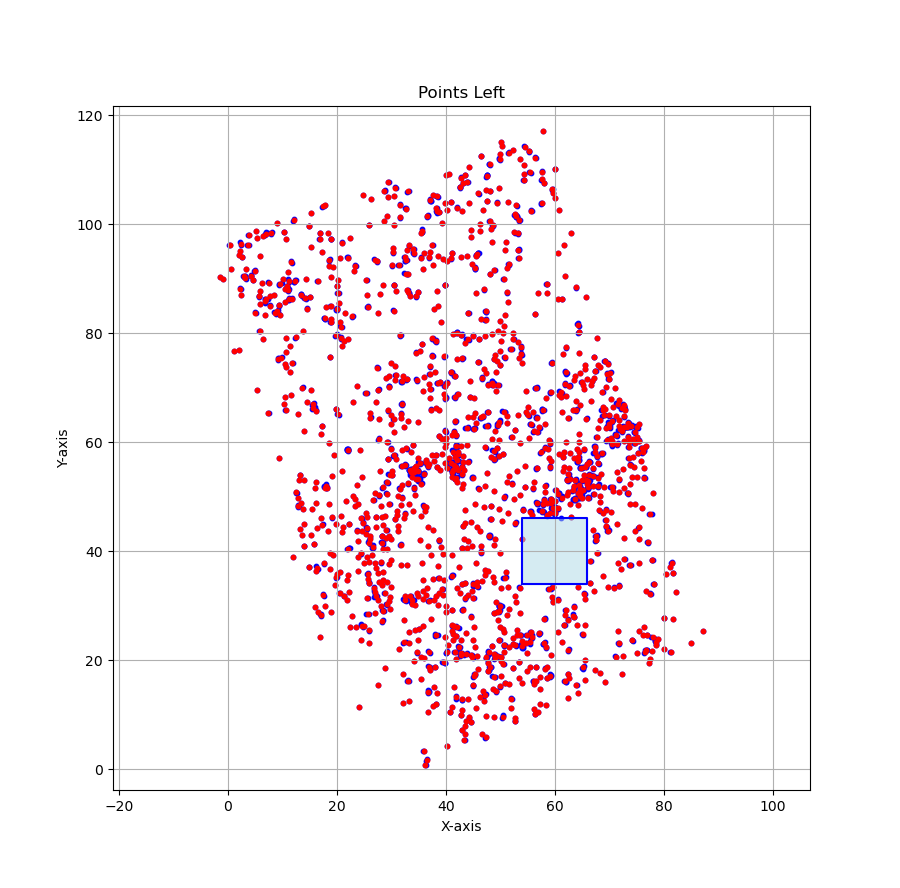
\includegraphics[height=36mm,width=0.24\textwidth]{Images/simulation_obs/Data/1.png}
% % %         & 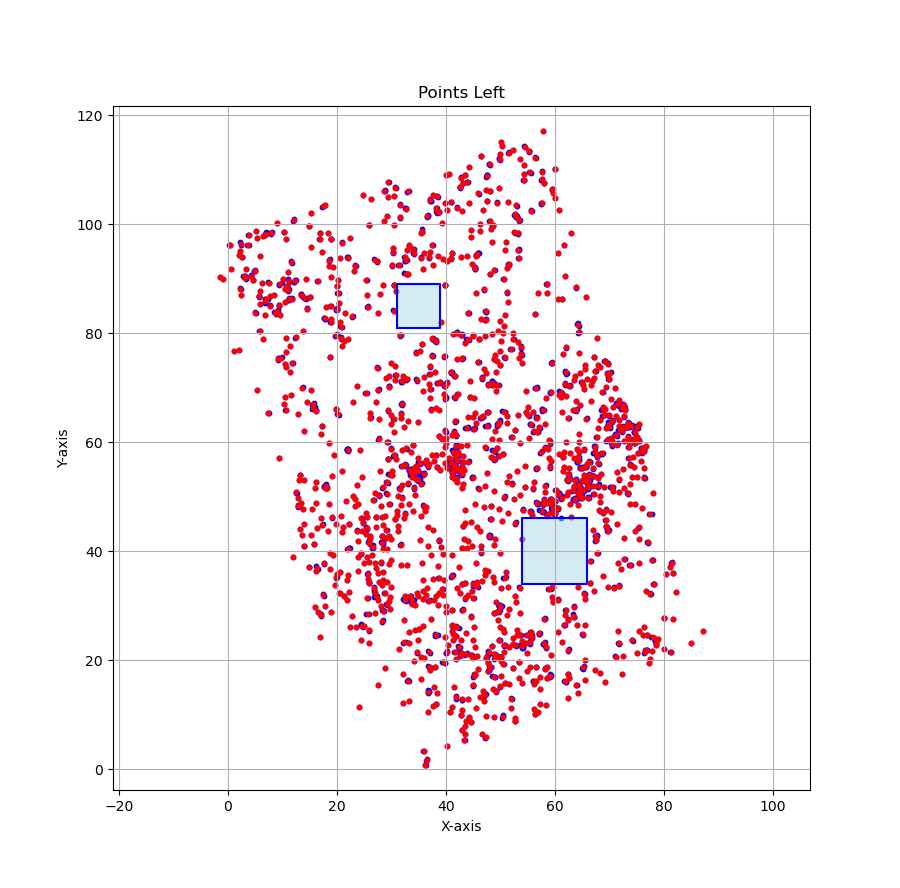
\includegraphics[height=36mm,width=0.24\textwidth]{Images/simulation_obs/Data/2.png}
% % %          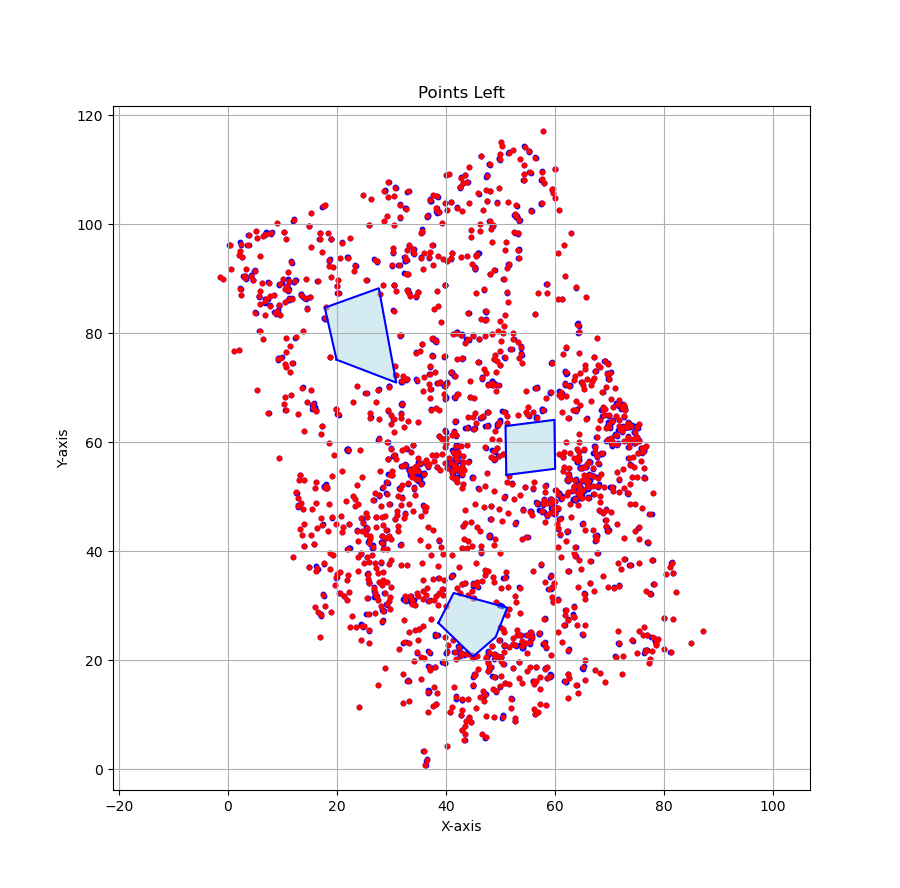
\includegraphics[height=36mm,width=0.24\textwidth]{Images/simulation_obs/Data/3.png}\\[-4pt]

% % %         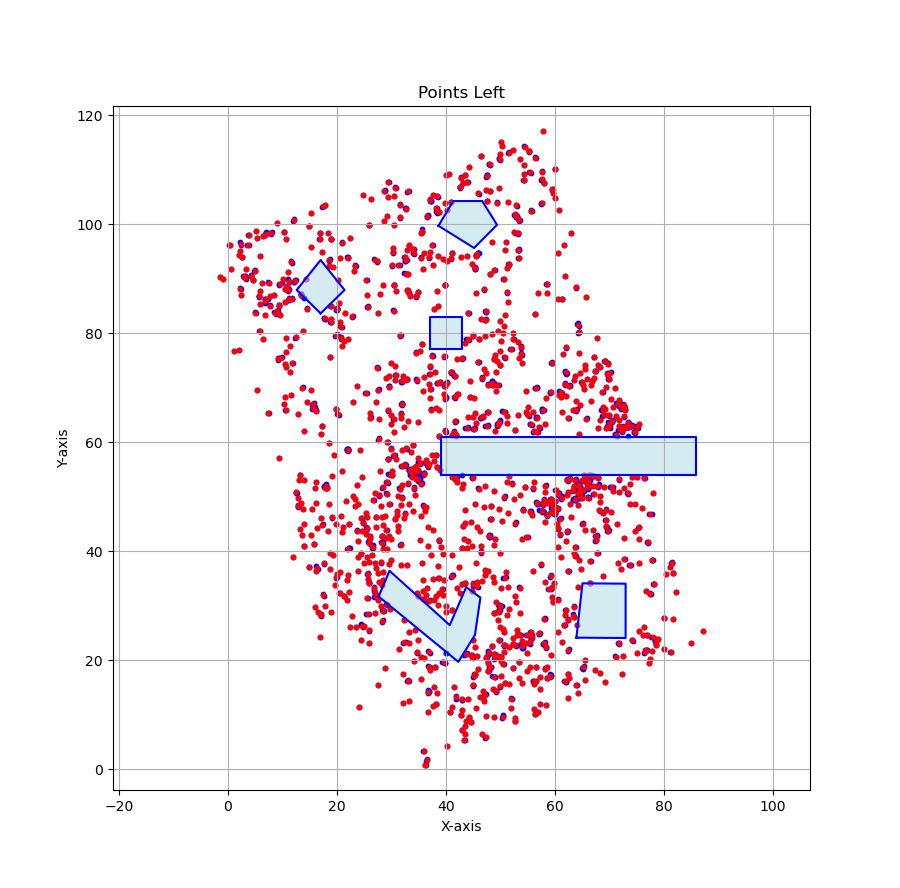
\includegraphics[height=36mm,width=0.24\textwidth]{Images/simulation_obs/Data/4.png}
% % %         & 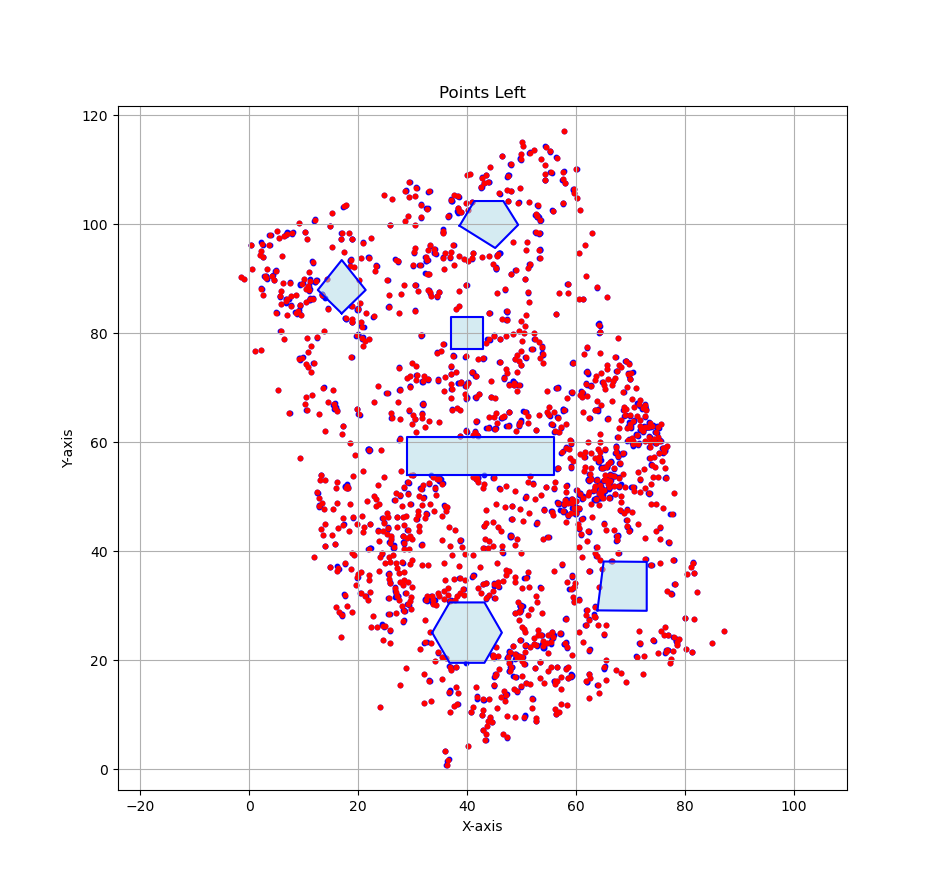
\includegraphics[height=36mm,width=0.24\textwidth]{Images/simulation_obs/Data/5.png}

% % %     \end{tabular}
% % %     \caption{Obstacles Dataset.\label{fig:obstacles_dataset}}
% % % \end{figure}


\vspace*{6mm}  



\subsection{Simulation Results and Analysis}

This section details the results and analysis of simulation experiments designed to evaluate the robustness of the proposed complete coverage path planning algorithm in the presence of static polygonal obstacles. The empirical findings are meticulously analyzed to provide insights into the algorithm's performance across diverse scenarios, offering a comprehensive assessment of its efficiency and effectiveness.

\vspace*{6mm}  

\textbf{Experimental Consistency}
To ensure the validity of comparisons and isolate the effects of different datasets on the algorithm's performance, the initial position and orientation of the robot were kept constant throughout all experiments. Additionally, the parameters for both the robot and the algorithm were consistently maintained across all trials.

\vspace*{6mm}  

\textbf{Robot Constraints and Algorithm Parameters: } 


The robot's constraints and operational parameters are set to realistic values to ensure the validity of the simulation results. These data can be visualized in (\autoref{tab:constraints_and_parameters_obs}).

% % % % Table robot parameters 1
% % % \begin{table}[]
% % %     \centering
% % %     \caption{Constraints and Parameters in presence of obstacles.}
% % %     \label{tab:constraints_and_parameters_obs}
% % %     \begin{tabular}{|c|c|}
% % %     \hline
% % %     \rowcolor[HTML]{FFCC67} 
% % %     \textit{\textbf{Constraints and Parameters}}                                    & \textit{\textbf{Values}}       \\ \hline
% % %     \rowcolor[HTML]{CBF9FC} 
% % %     \textit{Robot initial position}                                                 & {[}60.0, 1.0{]}                \\ \hline
% % %     \rowcolor[HTML]{CBF9FC} 
% % %     \textit{Robot initial orientation}                                              & 45                             \\ \hline
% % %     \rowcolor[HTML]{CBF9FC} 
% % %     \textit{Search angle of the vision cone}                                        & ±11                            \\ \hline
% % %     \rowcolor[HTML]{CBF9FC} 
% % %     \textit{Minimum search radius of the vision cone.}                              & 1.25                           \\ \hline
% % %     \rowcolor[HTML]{CBF9FC} 
% % %     \textit{Maximum search radius of the vision cone.}                              & 100                            \\ \hline
% % %     \rowcolor[HTML]{CBF9FC} 
% % %     \textit{Minimum turning radius allowed for the robot.}                          & 2.0                            \\ \hline
% % %     \rowcolor[HTML]{CBF9FC} 
% % %     \textit{robot velocity on curved paths.}                                        & 0.4                            \\ \hline
% % %     \rowcolor[HTML]{CBF9FC} 
% % %     \textit{robot velocity on straight paths.}                                      & 0.8                            \\ \hline
% % %     \rowcolor[HTML]{CBF9FC} 
% % %     \textit{Distance used to compute field time taken on curved paths.}             & 7.85                           \\ \hline
% % %     \rowcolor[HTML]{CBF9FC} 
% % %     \textit{Number of points to consider in the vision cone.}                       & 5                              \\ \hline
% % %     \rowcolor[HTML]{CBF9FC} 
% % %     \textit{Minimum distance between intermediate points, and start and end point.} & 2.7                            \\ \hline
% % %     \rowcolor[HTML]{CBF9FC} 
% % %     \textit{Minimum distance between intermediate points.}                          & 2                              \\ \hline
% % %     \rowcolor[HTML]{CBF9FC} 
% % %     \textit{Maximum distance of the intermediate point form the path.}              & 0.6                            \\ \hline
% % %     \rowcolor[HTML]{CBF9FC} 
% % %     \textit{Graph search extreme angles}                                            & ±11                            \\ \hline
% % %     \rowcolor[HTML]{CBF9FC} 
% % %     \textit{buffer distance around obstacles.}                                      & 1                              \\ \hline
% % %     \rowcolor[HTML]{CBF9FC} 
% % %     \textit{Extend polygon distance for safe region.}                               & 1.4                            \\ \hline
% % %     \rowcolor[HTML]{CBF9FC} 
% % %     \textit{Graph generation step reduction iteration.}                             & 3                              \\ \hline
% % %     \rowcolor[HTML]{CBF9FC} 
% % %     \textit{Grid diameter.}                                                         & 0.4                            \\ \hline
% % %     \rowcolor[HTML]{CBF9FC} 
% % %     \textit{Max generation for graph generation.}                                   & 18                             \\ \hline
% % %     \rowcolor[HTML]{CBF9FC} 
% % %     \textit{Minimum step length for graph generation.}                              & 1.2                            \\ \hline
% % %     \rowcolor[HTML]{CBF9FC} 
% % %     \textit{Total operational area.}                                                & {[}{[}-2,0{]}, {[}90,120{]}{]} \\ \hline
% % %     \rowcolor[HTML]{CBF9FC} 
% % %     \textit{Distance between waypoints.}                                            & 10                             \\ \hline
% % %     \end{tabular}
% % %     \end{table}


The algorithm parameters are also meticulously defined to ensure consistent performance across all experiments. These parameters are set based on the robot's physical constraints and operational requirements, ensuring that the algorithm operates within realistic boundaries.

\vspace*{6mm} 

The algorithm was designed to initially compute the global coverage path using straight lines. Subsequently, Dubins paths are generated for each line segment to ensure the shortest feasible path between each pair of points, optimizing the overall path length. The (\autoref{fig:straight_path_obs}) illustrate the straight obstacle free paths generated by the algorithm for all the datasets.

% % % % Straight_path with obstacles   
% % % \begin{figure}[]
% % %     \centering
% % %     \begin{tabular}{ccc} 
% % %          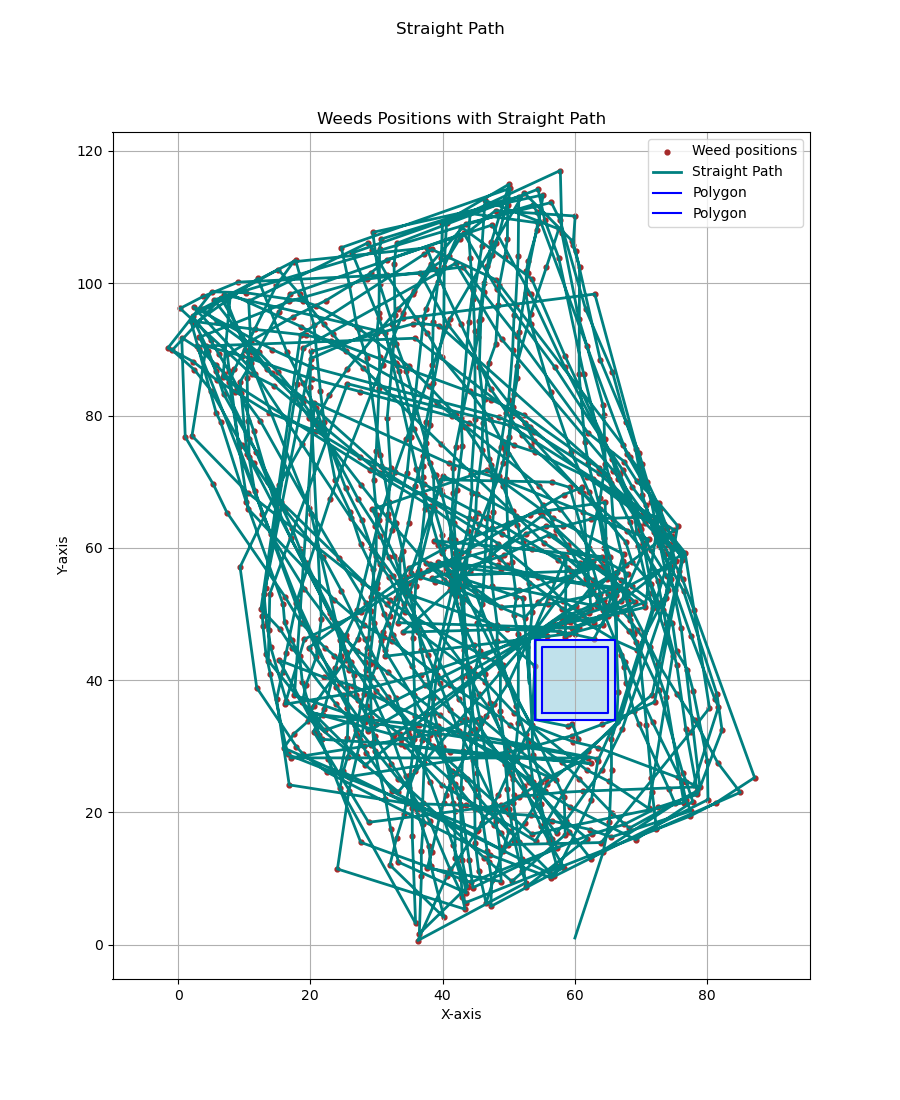
\includegraphics[height=36mm,width=0.24\textwidth]{Images/simulation_obs/obs_straight/1.png}
% % %         & 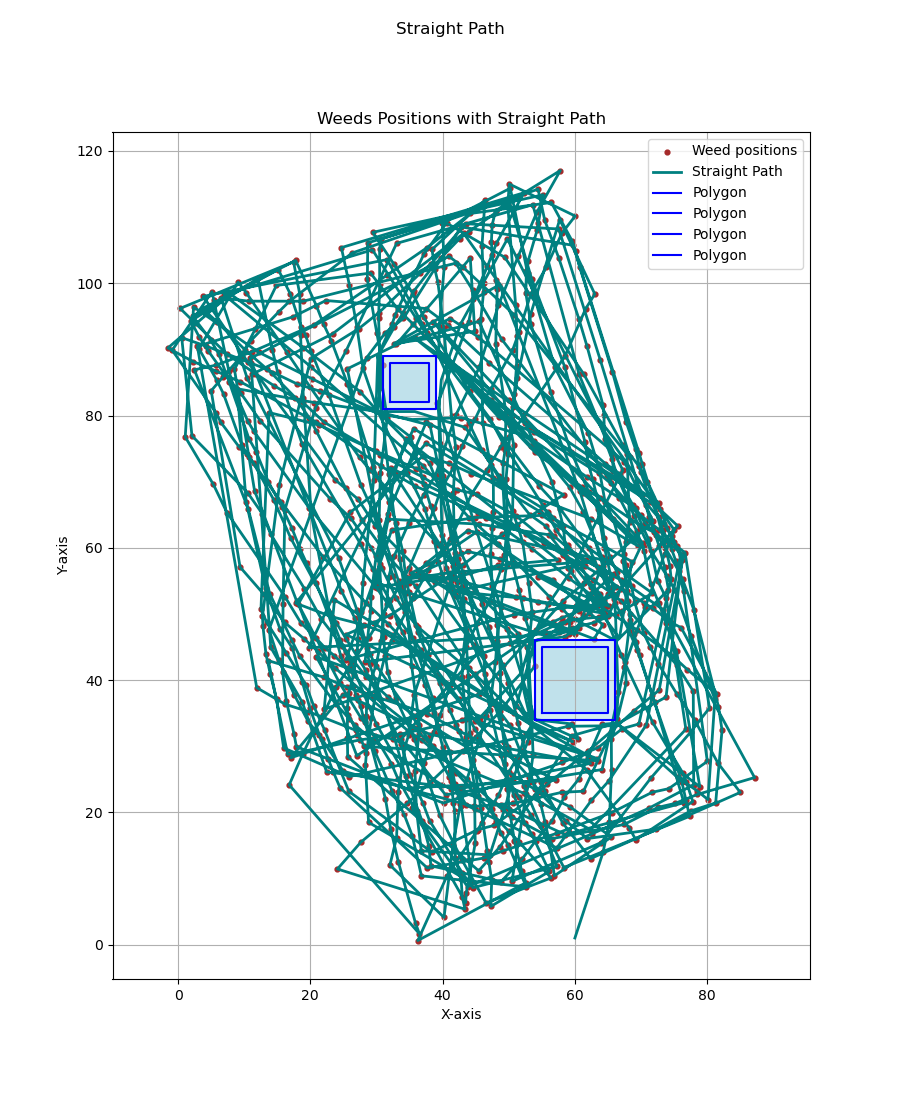
\includegraphics[height=36mm,width=0.24\textwidth]{Images/simulation_obs/obs_straight/2.png}
% % %          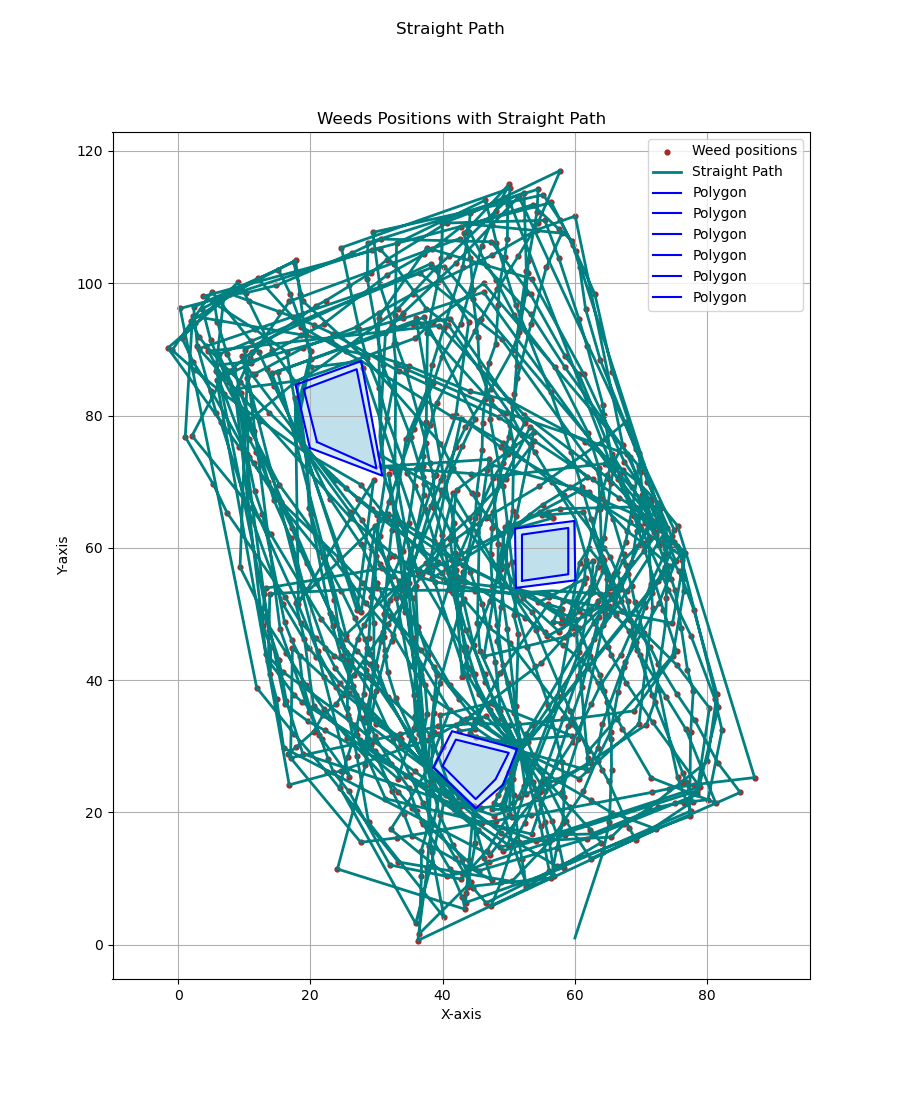
\includegraphics[height=36mm,width=0.24\textwidth]{Images/simulation_obs/obs_straight/3.png}\\[-4pt]

% % %         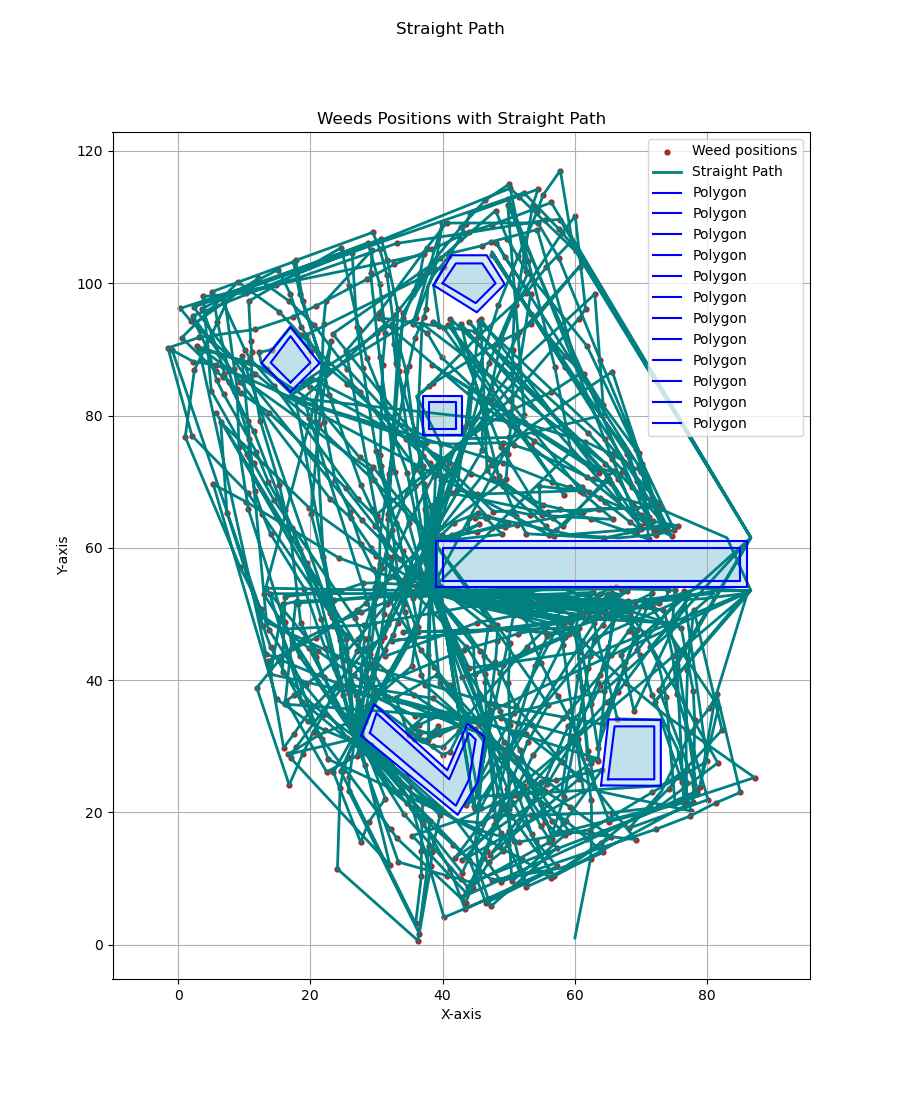
\includegraphics[height=36mm,width=0.24\textwidth]{Images/simulation_obs/obs_straight/4.png}
% % %         & 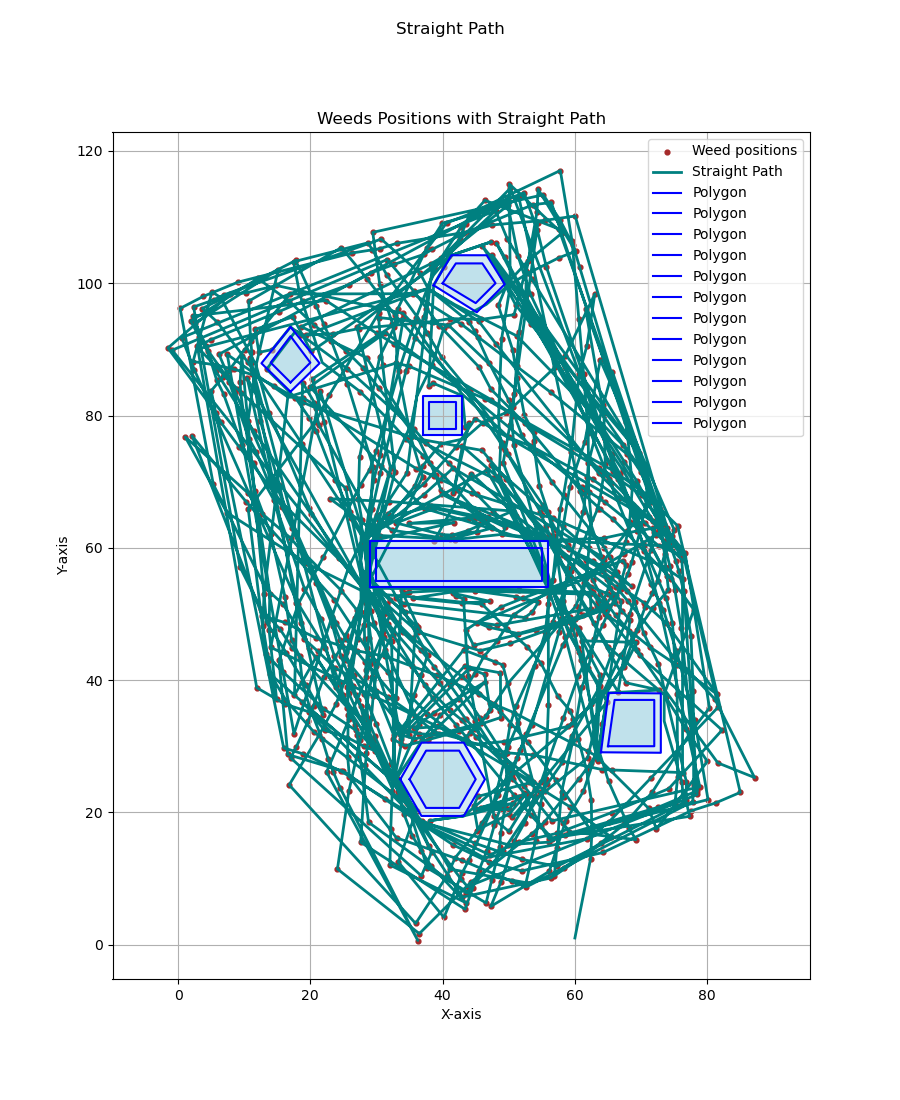
\includegraphics[height=36mm,width=0.24\textwidth]{Images/simulation_obs/obs_straight/5.png} 

% % %     \end{tabular}
% % %     \caption{Straight Path.\label{fig:straight_path_obs}}
% % % \end{figure}


\vspace*{6mm}

The resulting path after applying dubins constraints are depicted in the (\autoref{fig:dubins_path_obs}). These visual representations portray the robot's movement across diverse datasets, providing insight into the algorithm's adaptability amidst varying obstacles. 



% % % % Dubins_path with obstacles   
% % % \begin{figure}[htbp]
% % %     \centering
% % %     \begin{tabular}{ccc} 
% % %          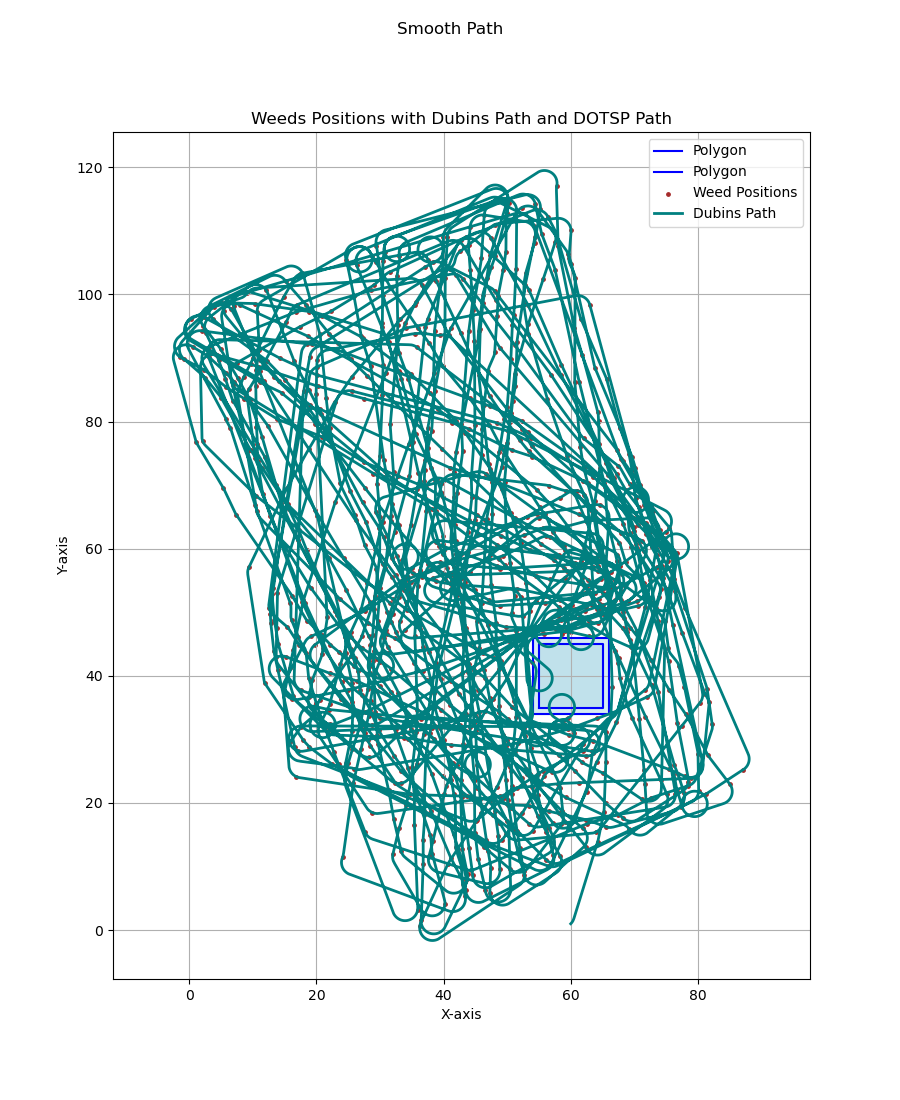
\includegraphics[height=36mm,width=0.24\textwidth]{Images/simulation_obs/obs_dubins/1.png}
% % %         & 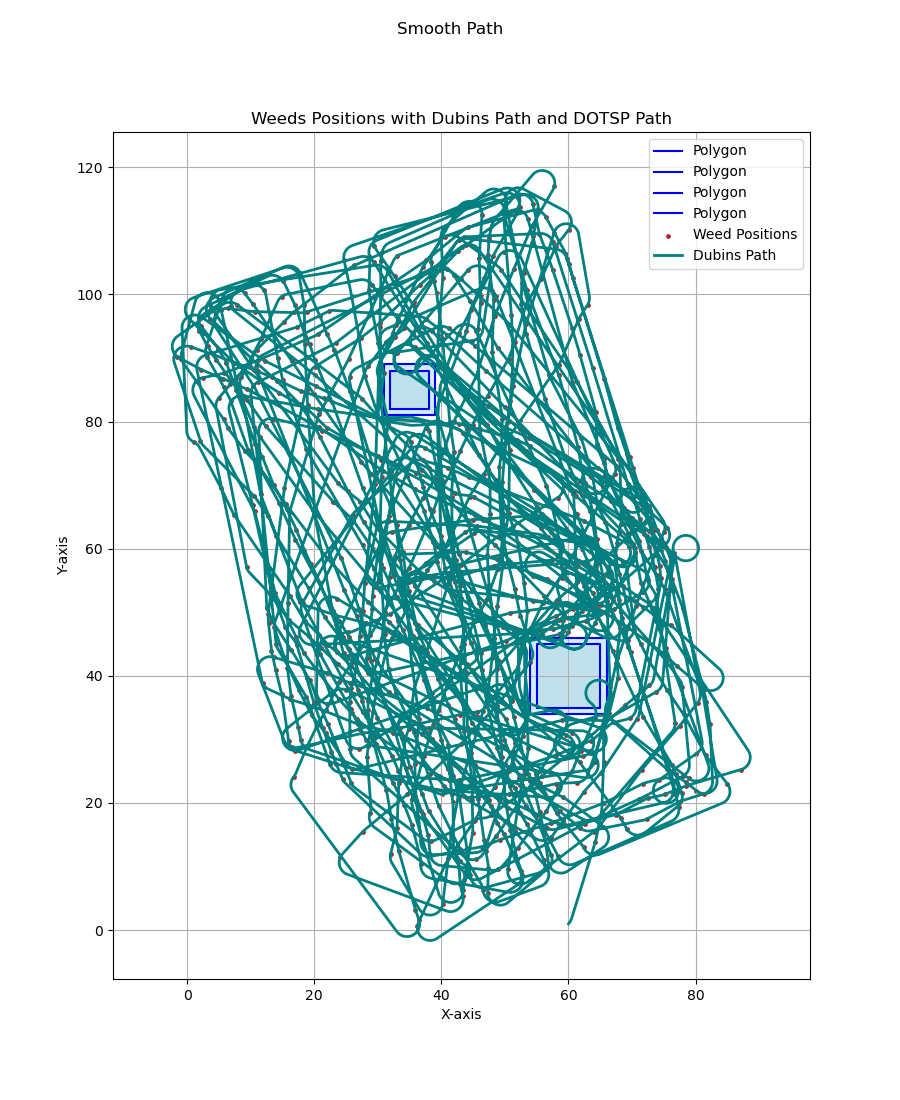
\includegraphics[height=36mm,width=0.24\textwidth]{Images/simulation_obs/obs_dubins/2.png}
% % %          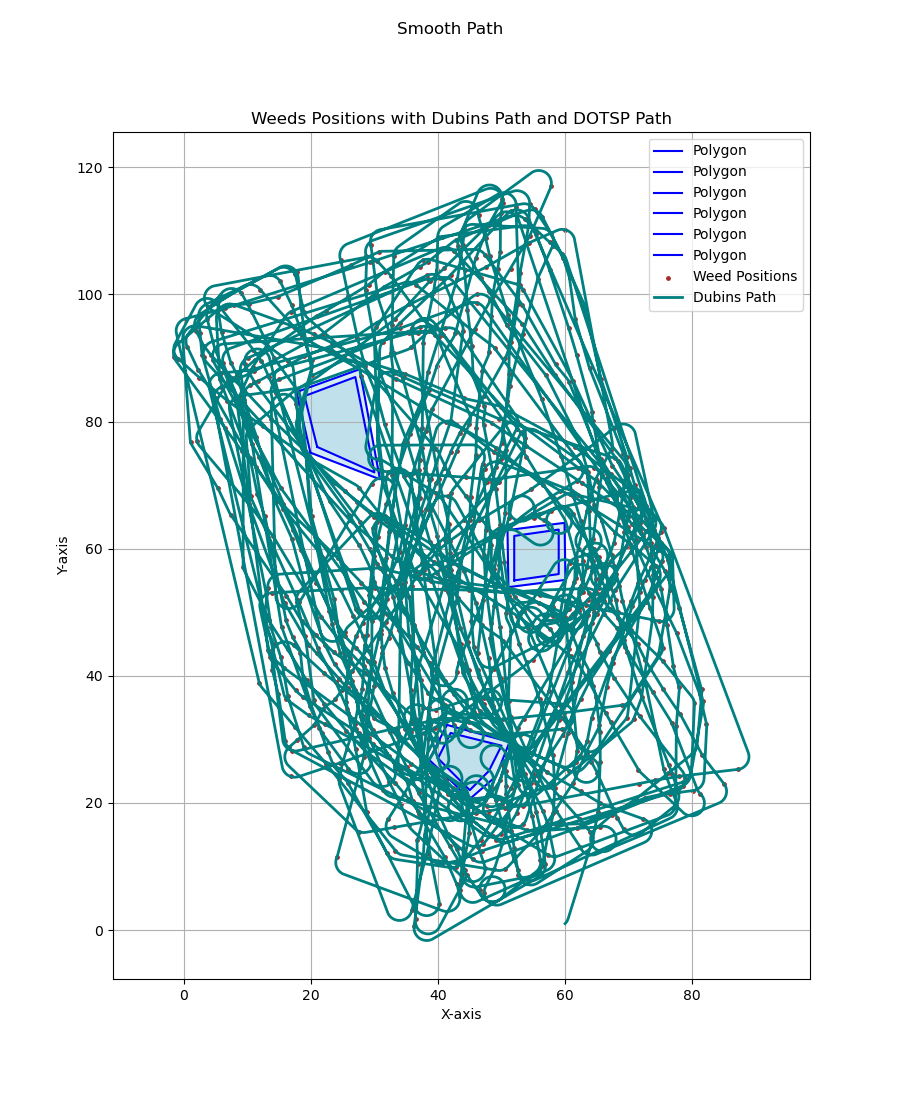
\includegraphics[height=36mm,width=0.24\textwidth]{Images/simulation_obs/obs_dubins/3.png}\\[-4pt]

% % %         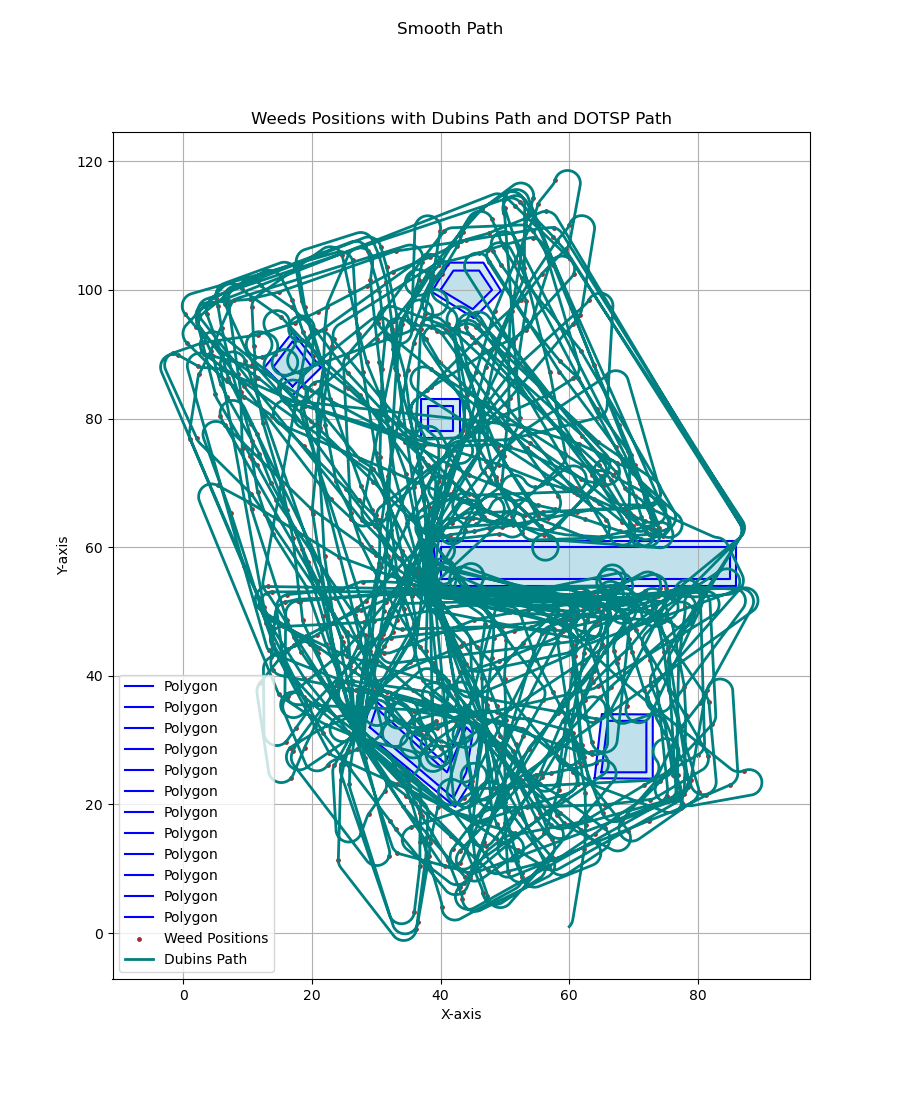
\includegraphics[height=36mm,width=0.24\textwidth]{Images/simulation_obs/obs_dubins/4.png}
% % %         & 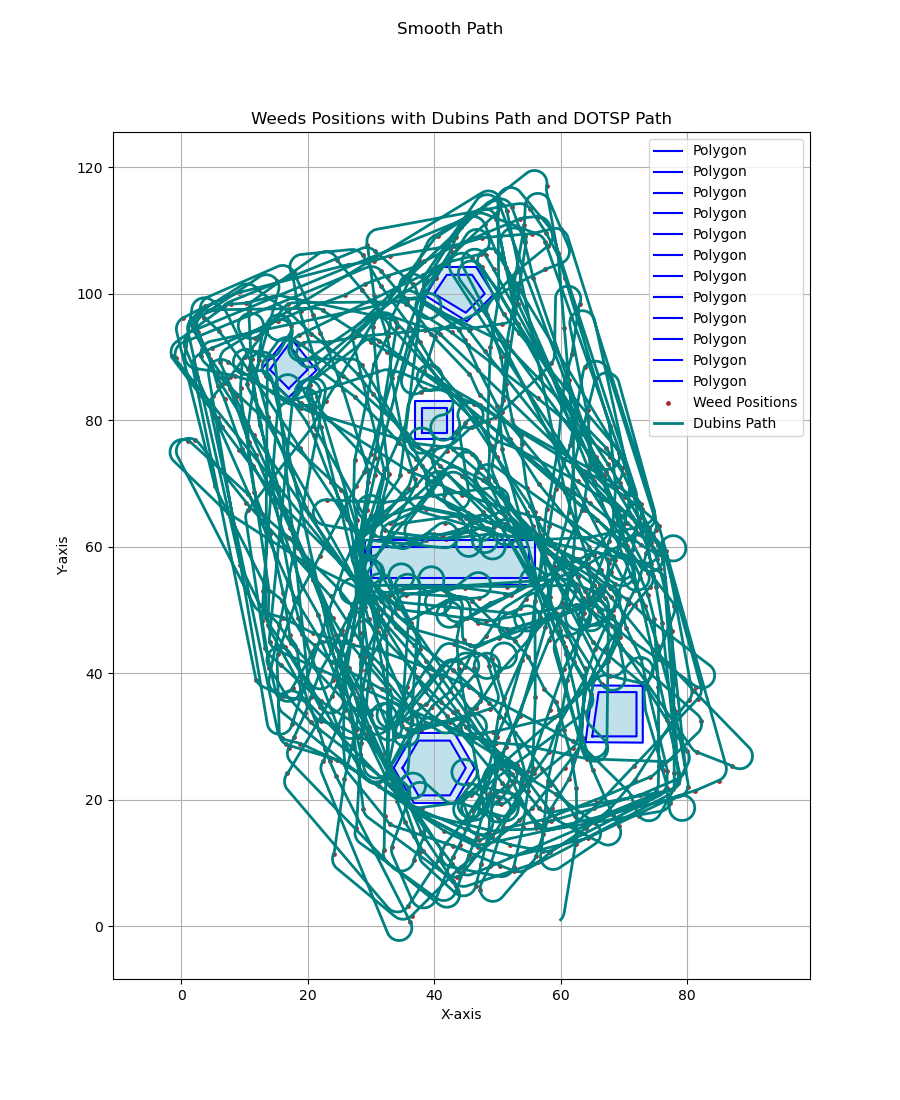
\includegraphics[height=36mm,width=0.24\textwidth]{Images/simulation_obs/obs_dubins/5.png} 

% % %     \end{tabular}
% % %     \caption{Dubins' Path.\label{fig:dubins_path_obs}}
% % % \end{figure}

\vspace*{6mm}  

The (\autoref{tab:performance_metrics_obs}) summarizes the performance metrics for all datasets, offering valuable insights into the algorithm's computational efficiency, operational effectiveness, and overall robustness.

% % % Table for perfromance metrics with obstacles
% % \begin{table}[H]
% %     \centering
% %     \caption{Results for the performance metrics.}
% %     \label{tab:performance_metrics_obs}
% %     \begin{tabular}{llllll}
% %     \hline
% %     \rowcolor[HTML]{67D5DA} 
% %     \textit{\textbf{Cases}} & \textit{\textbf{\begin{tabular}[c]{@{}l@{}}Computation \\ Time in secs.\end{tabular}}} & \textit{\textbf{\begin{tabular}[c]{@{}l@{}}Field Operation\\  Time in sec.\end{tabular}}} & \textit{\textbf{\begin{tabular}[c]{@{}l@{}}Route length\\  in meters\end{tabular}}} & \textit{\textbf{\begin{tabular}[c]{@{}l@{}}No. of \\ Turns.\end{tabular}}} & \textit{\textbf{\begin{tabular}[c]{@{}l@{}}Energy \\ Consumption \\ in KWh.\end{tabular}}} \\ \hline
% %     \rowcolor[HTML]{FFFFC7} 
% %     case 1                  & 13.32                                                                                  & 14612.4                                                                                   & 10637.003                                                                           & 134                                                                        & 13792.7026                                                                                 \\ \hline
% %     \rowcolor[HTML]{FFFFC7} 
% %     case 2                  & 20.762                                                                                 & 15170.4                                                                                   & 11028.086                                                                           & 141                                                                        & 14348.6364                                                                                 \\ \hline
% %     \rowcolor[HTML]{FFFFC7} 
% %     case 3                  & 35.71                                                                                  & 15094.8                                                                                   & 11079.932                                                                           & 127                                                                        & 14070.7815                                                                                 \\ \hline
% %     \rowcolor[HTML]{FFFFC7} 
% %     case 4                  & 93.918                                                                                 & 18694.8                                                                                   & 13738.529                                                                           & 155                                                                        & 17388.7787                                                                                 \\ \hline
% %     \rowcolor[HTML]{FFFFC7} 
% %     case 5                  & 58.307                                                                                 & 16160.4                                                                                   & 12010.546                                                                           & 117                                                                        & 14765.8961                                                                                 \\ \hline
% %     \end{tabular}
% %     \end{table}

\vspace*{6mm}

Additionally, the coverage rate plot over the field time provides a visual depiction of the algorithm's performance across all datasets. This plot illustrates how efficiently the algorithm achieves coverage over time, facilitating a comparative analysis of its efficiency under varying scenarios. Please refer to (\autoref{fig:coverage_plots_obs}) for visualization of the coverage plots.

% % % % coverage plots with obstacles   
% % % \begin{figure}[H]
% % %     \centering
% % %     \begin{tabular}{ccc} 
% % %          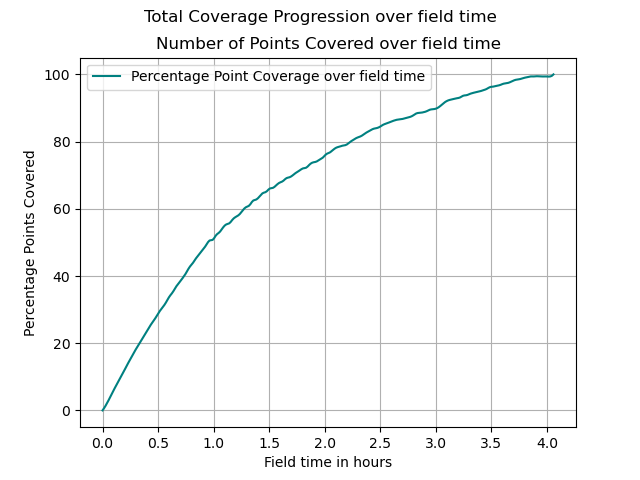
\includegraphics[height=36mm,width=0.24\textwidth]{Images/simulation_obs/coverage_plots/1.png}
% % %         & 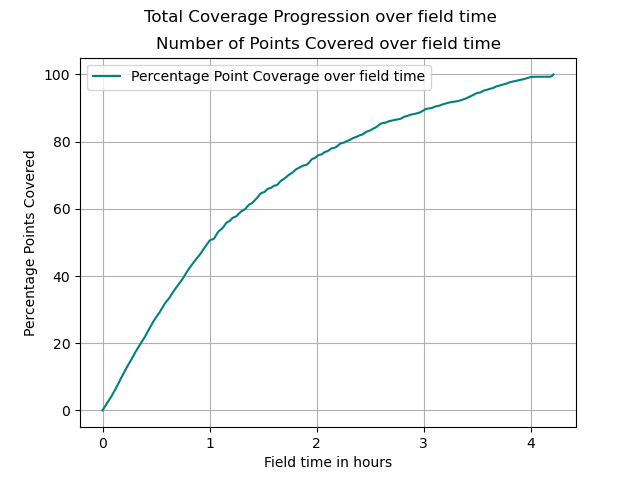
\includegraphics[height=36mm,width=0.24\textwidth]{Images/simulation_obs/coverage_plots/2.png}
% % %          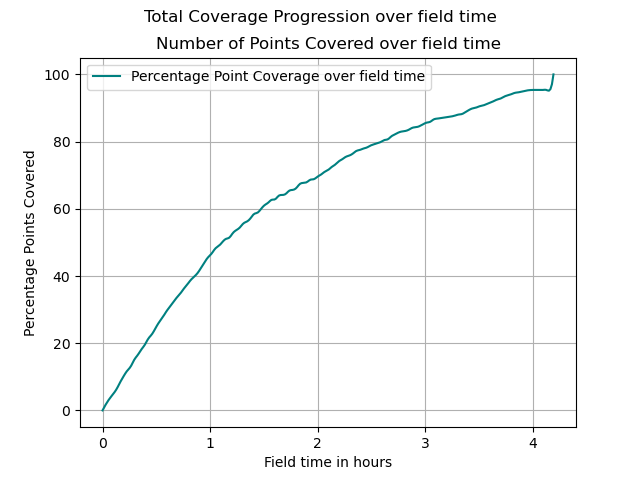
\includegraphics[height=36mm,width=0.24\textwidth]{Images/simulation_obs/coverage_plots/3.png}\\[-4pt]

% % %         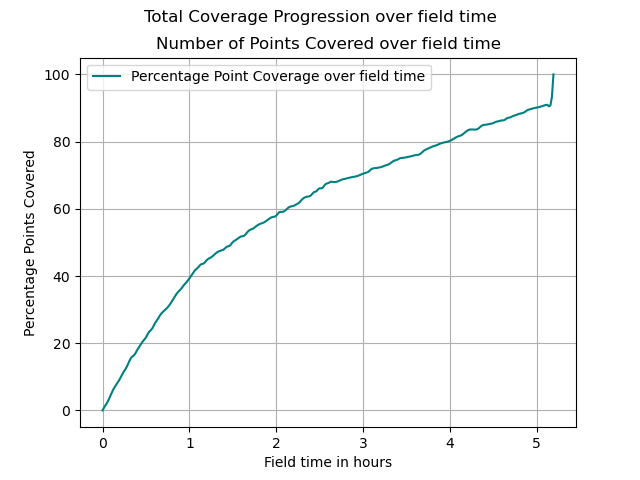
\includegraphics[height=36mm,width=0.24\textwidth]{Images/simulation_obs/coverage_plots/4.png}
% % %         & 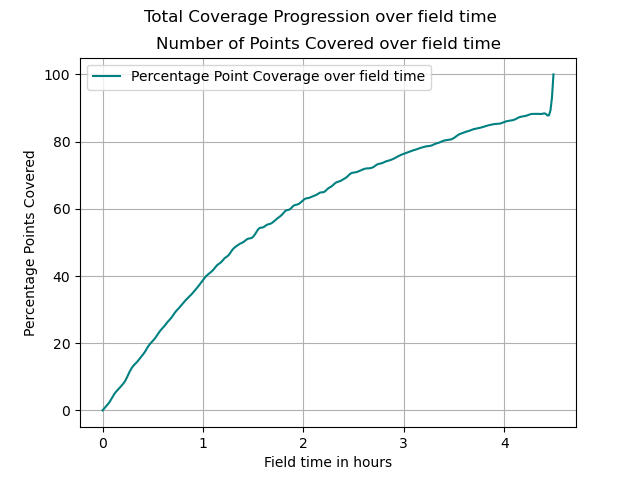
\includegraphics[height=36mm,width=0.24\textwidth]{Images/simulation_obs/coverage_plots/5.png} 

% % %     \end{tabular}
% % %     \caption{Coverage plots.\label{fig:coverage_plots_obs}} 
% % % \end{figure}


The remaining points after the completion of the second behavior in presence of obstacles are depicted in the (\autoref{fig:remaining_points_obs}). 

% % % % remaining points with obstacles   
% % % \begin{figure}[H]
% % %     \centering
% % %     \begin{tabular}{ccc} 
% % %          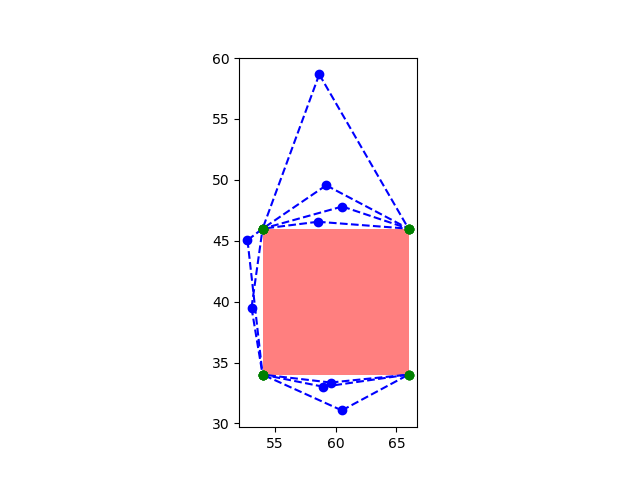
\includegraphics[height=36mm,width=0.24\textwidth]{Images/simulation_obs/left_points_near_obs/1.png}
% % %         & 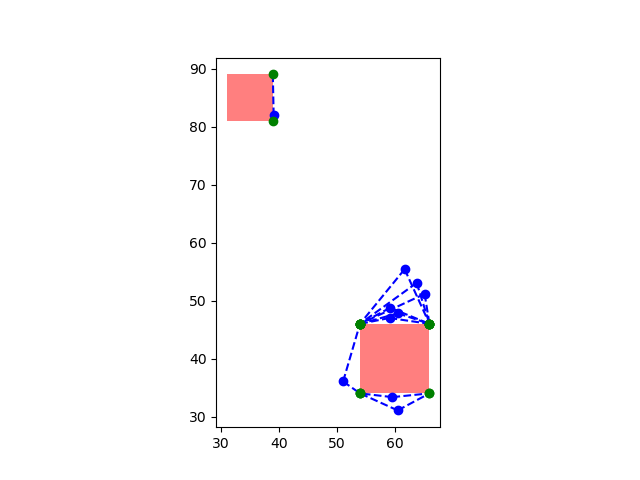
\includegraphics[height=36mm,width=0.24\textwidth]{Images/simulation_obs/left_points_near_obs/2.png}
% % %          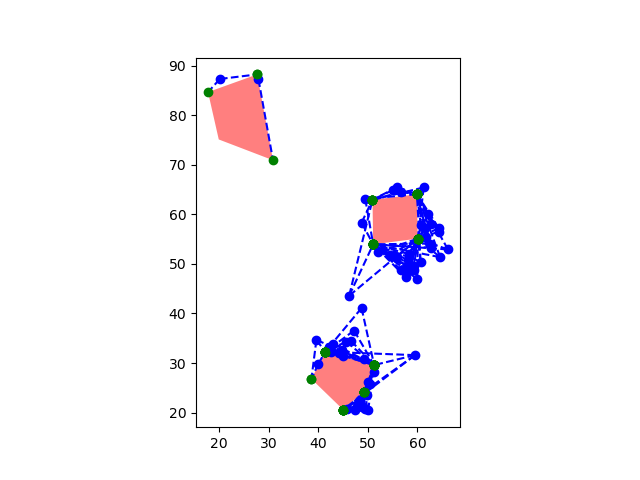
\includegraphics[height=36mm,width=0.24\textwidth]{Images/simulation_obs/left_points_near_obs/3.png}\\[-4pt]

% % %         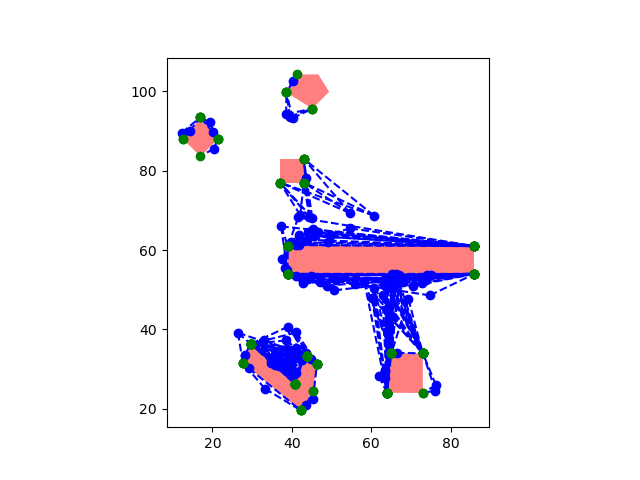
\includegraphics[height=36mm,width=0.24\textwidth]{Images/simulation_obs/left_points_near_obs/4.png}
% % %         & 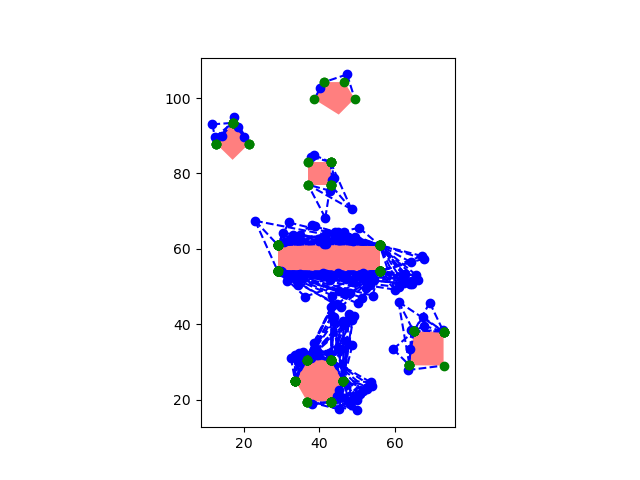
\includegraphics[height=36mm,width=0.24\textwidth]{Images/simulation_obs/left_points_near_obs/5.png} 

% % %     \end{tabular}
% % %     \caption{Remaining points after second behavior.\label{fig:remaining_points_obs}} 
% % % \end{figure}

The path obtained for the remaining points utiizing the third behavior can be visualized in the (\autoref{fig:remaining_path_obs}). 

% % % % remaining points path with obstacles   
% % % \begin{figure}[H]
% % %     \centering
% % %     \begin{tabular}{ccc} 
% % %          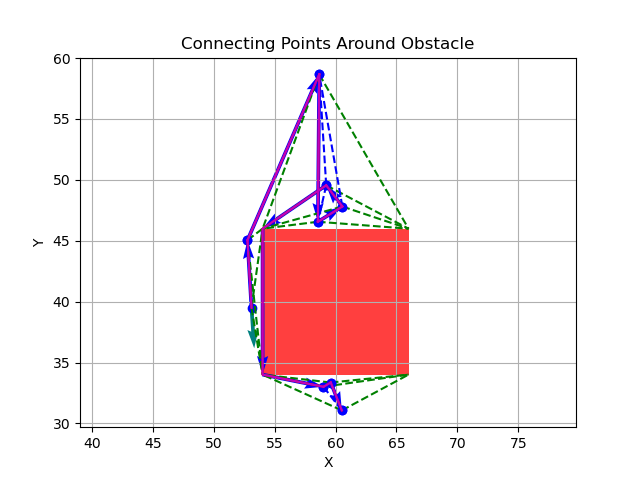
\includegraphics[height=36mm,width=0.24\textwidth]{Images/simulation_obs/left_points_covered_obs/1.png}
% % %         & 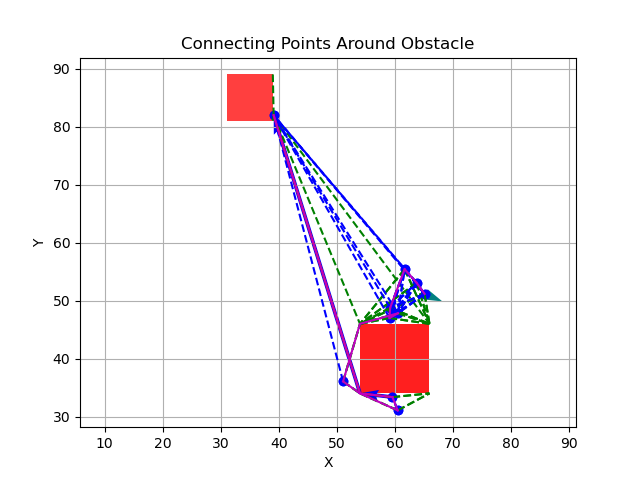
\includegraphics[height=36mm,width=0.24\textwidth]{Images/simulation_obs/left_points_covered_obs/2.png}
% % %          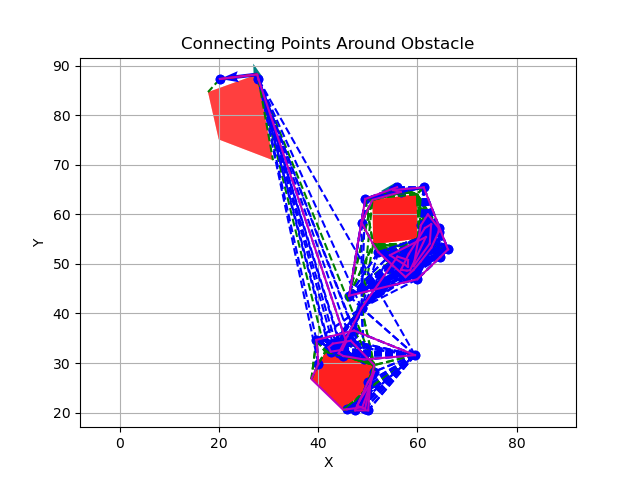
\includegraphics[height=36mm,width=0.24\textwidth]{Images/simulation_obs/left_points_covered_obs/3.png}\\[-4pt]

% % %         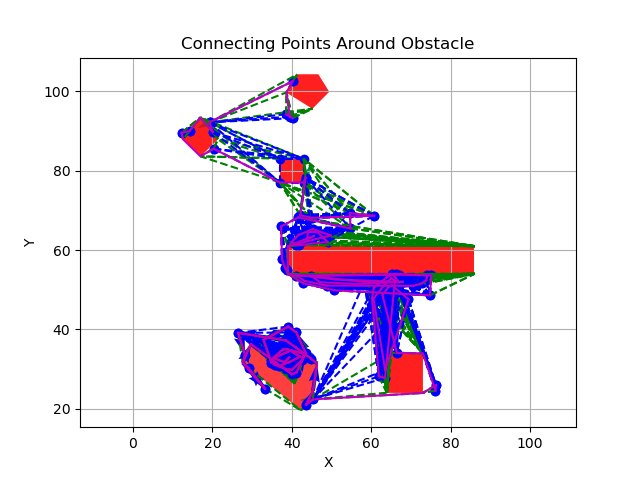
\includegraphics[height=36mm,width=0.24\textwidth]{Images/simulation_obs/left_points_covered_obs/4.png}
% % %         & 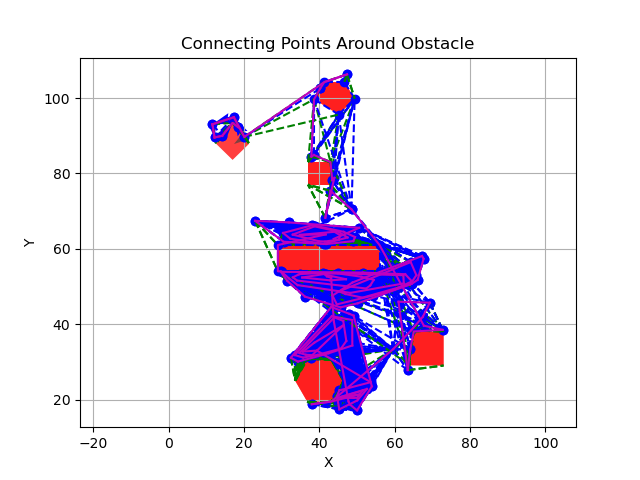
\includegraphics[height=36mm,width=0.24\textwidth]{Images/simulation_obs/left_points_covered_obs/5.png} 

% % %     \end{tabular}
% % %     \caption{Path for remaining points.\label{fig:remaining_path_obs}} 
% % % \end{figure}


Each perfromance metrics for all the datasets are plotted for better visualization and analysis of the algorithm's performance. The plots are depicted in the (\autoref{fig:Computation_time_obs}), (\autoref{fig:Energy_expenditure_obs}), (\autoref{fig:Route_length_obs}), (\autoref{fig:Field_operation_time_obs}), and (\autoref{fig:number_of_turns_obs}).


% \begin{figure}[H]
%     \centering
%     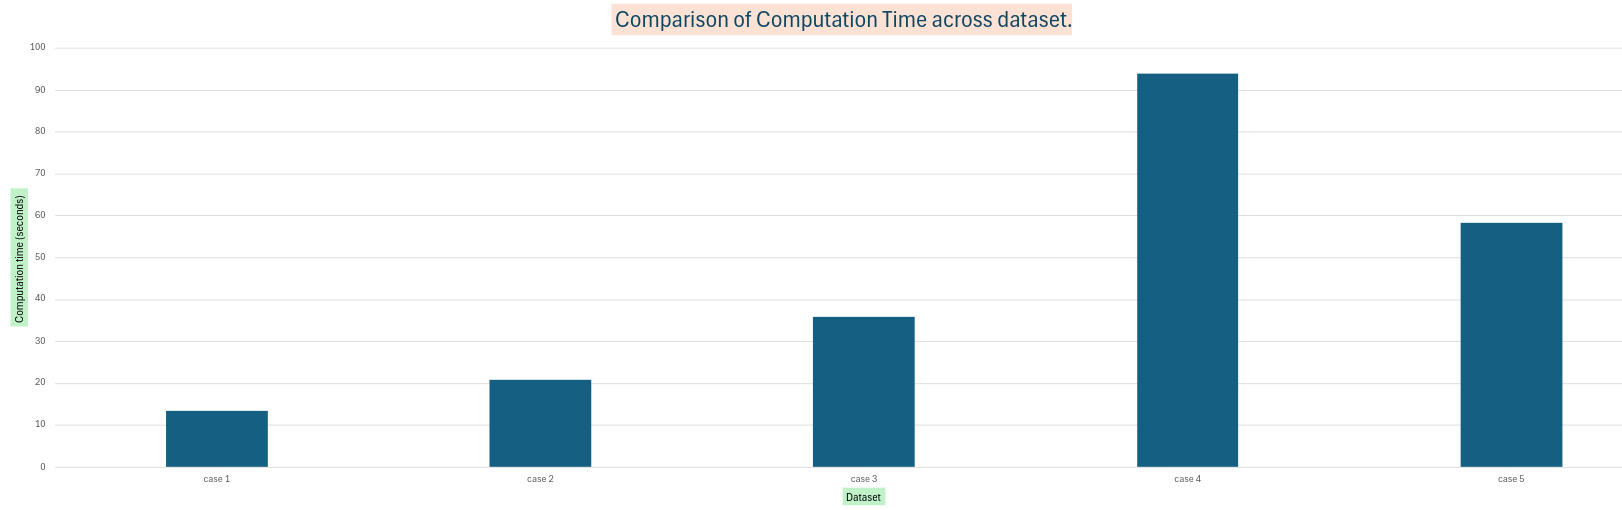
\includegraphics[width=\textwidth]{Images/plots/obs/computation_time.png}
%     \caption{Computation Time.}
%     \label{fig:Computation_time_obs}
% \end{figure}

% \begin{figure}[H]
%     \centering
%     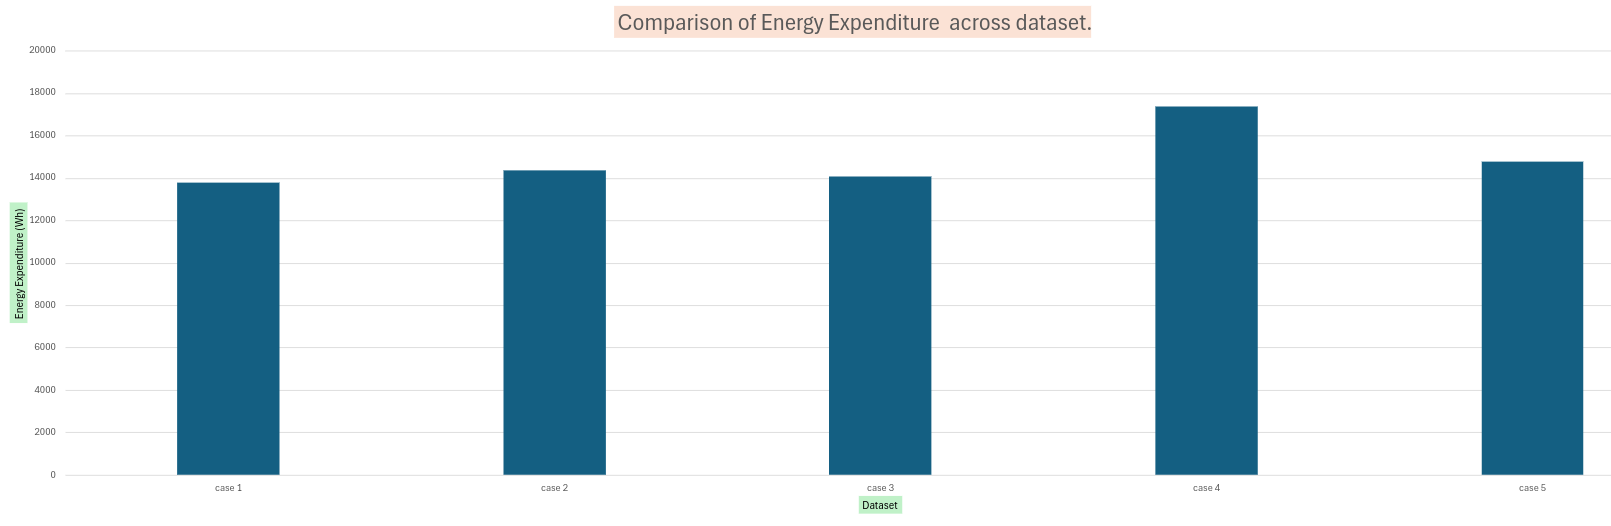
\includegraphics[width=\textwidth]{Images/plots/obs/Energy.png}
%     \caption{Energy Expenditure.}
%     \label{fig:Energy_expenditure_obs}
% \end{figure}

% \begin{figure}[H]
%     \centering
%     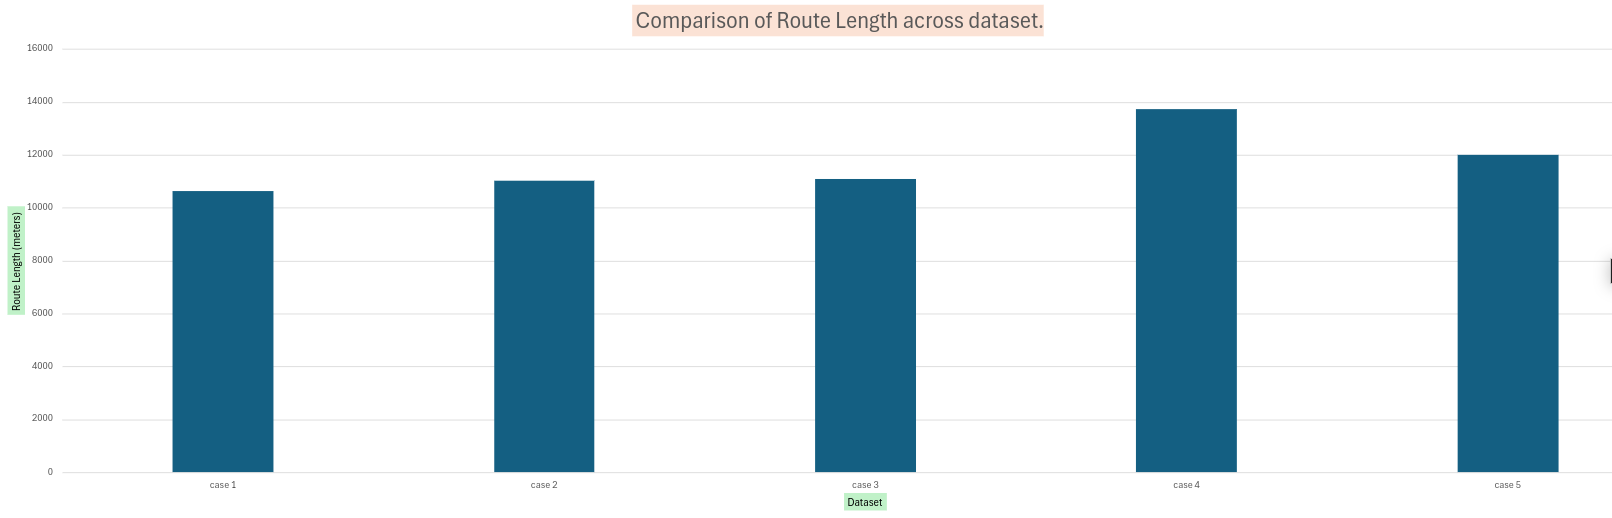
\includegraphics[width=\textwidth]{Images/plots/obs/route_length.png}
%     \caption{Route Length.}
%     \label{fig:Route_length_obs}
% \end{figure}

% \begin{figure}[H]
%     \centering
%     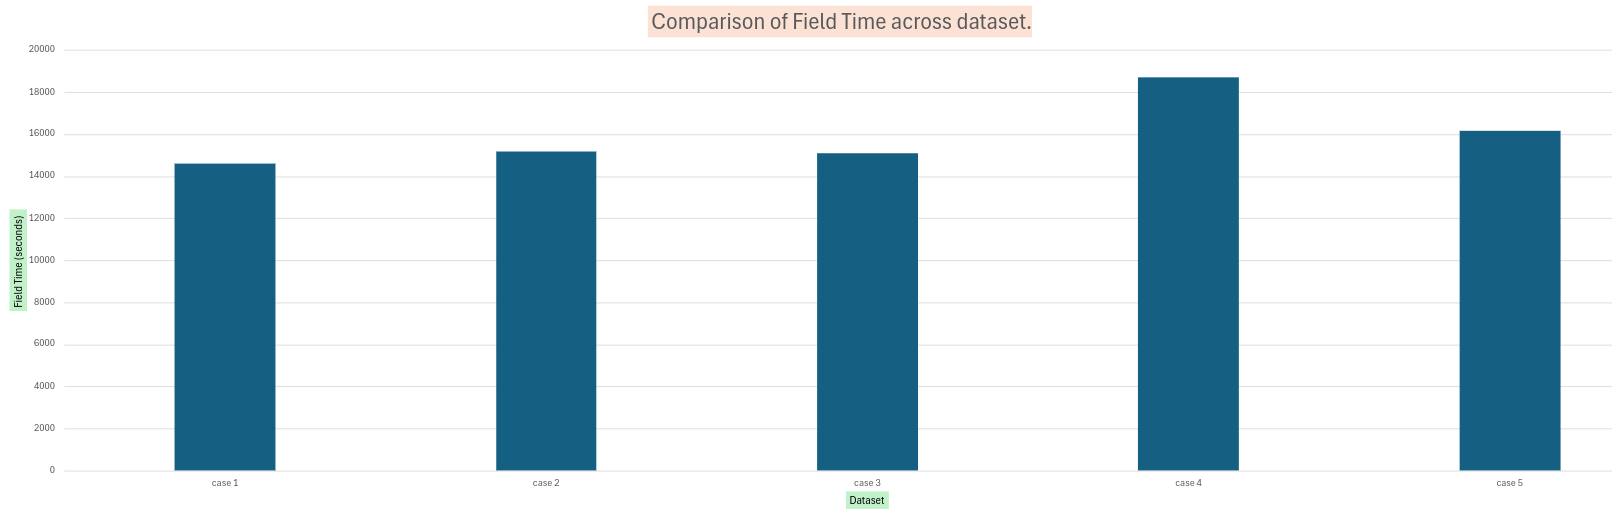
\includegraphics[width=\textwidth]{Images/plots/obs/Field time.png}
%     \caption{Field Operation Time.}
%     \label{fig:Field_operation_time_obs}
% \end{figure}

% \begin{figure}[H]
%     \centering
%     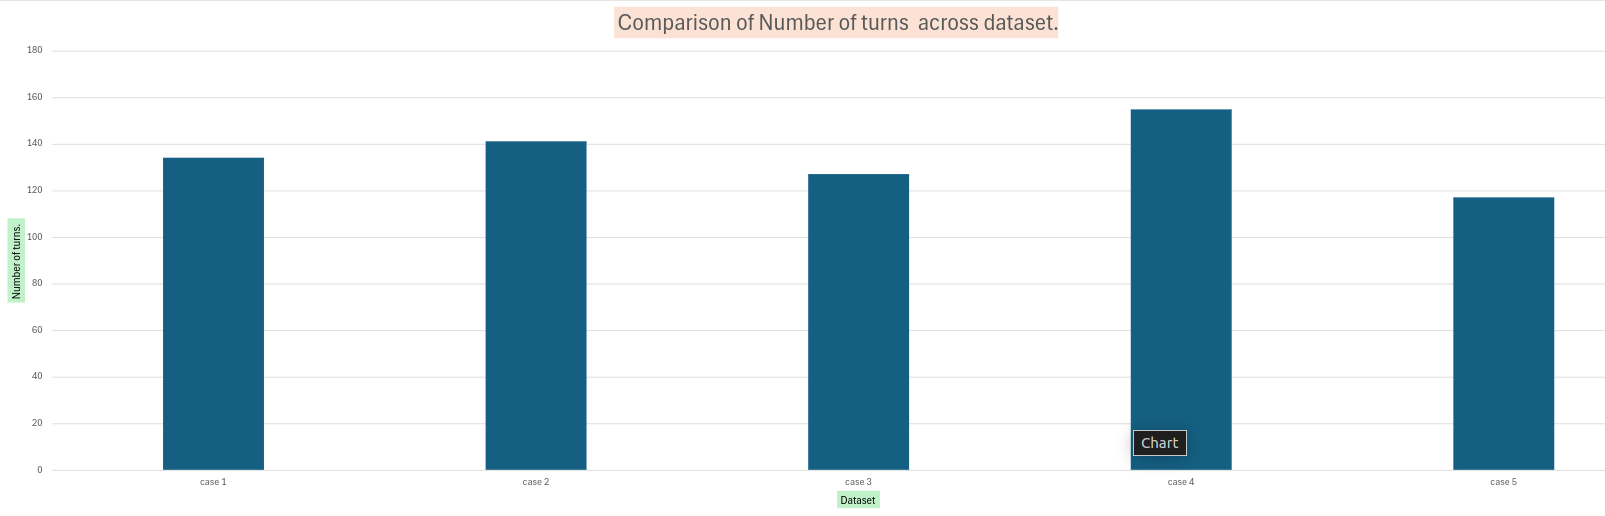
\includegraphics[width=\textwidth]{Images/plots/obs/Number of turns.png}
%     \caption{Number of Turns.}
%     \label{fig:number_of_turns_obs}
% \end{figure}


\textbf{Analysis: }

From the above plots for computational time, it is evident that computational time increases as the number and complexity of obstacles in the area increase. This is due to the hybrid space approach employed (combining continuous and discrete methods). As is well known, discrete approaches generally require more computation time compared to continuous methods. In our case, an increase in the number or size of obstacles results in a larger discrete space region, thereby increasing computational time. Additionally, as the number of obstacles increases, the likelihood of the path colliding with obstacles rises, necessitating repeated graph generation and path computation for each collision. Therefore, more obstacles and more complex shapes contribute to increased computational time.


\vspace*{6mm}

However, despite these challenges, the algorithm consistently computes paths within a reasonable timeframe. Even in the most extreme case (case 4, characterized by extensively large, convex, and concave obstacles), the maximum computation time recorded was 93.91 seconds (1.56 minutes). This is well within the acceptable range for agricultural field applications and demonstrates greater efficiency compared to most existing coverage path planning approaches with obstacle avoidance. The efficiency of the algorithm can be attributed to the automatic selection of the step length during graph generation, which is dynamically adjusted to expedite the process. Even in scenarios where frequent path collisions with obstacles occur, the algorithm adaptively modifies the step length to circumvent these obstacles, thereby reducing overall computation time.


\vspace*{6mm}

Regarding route length, energy expenditure, and field operation time, the results indicate that for the same data distribution with varying number and size of the obstacles, these performance metrics remain relatively consistent across different cases. This highlights the robustness of the algorithm; despite the increased number and complexity of obstacles, the algorithm can compute near-optimal, smooth, natural paths that minimize energy consumption, field operation time, and the number of turns.
